\chapter{Introduction}


\section{Motivation}
Automatic speech recognition(ASR) is one of the subfield of natural language processing(NLP) with many practical applications. Some examples of practical applications in speech recognition; for example: automatic closed captioning for hearing-disabled persons \cite{Patel2010}, taking notes of conversations between doctors and patients \cite{Klann2008}, automatic closed captioning TV broadcasts \cite{Woodland2015}, and many more.
This internship will focus on the application of automatic transcription on television broadcasts.

\begin{figure}[H]
\caption{automatic speech recognition}
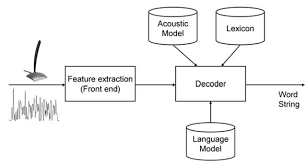
\includegraphics{asr}
\label{AutomaticSpeechRecognition}
\centering
\end{figure}

Picture \ref{AutomaticSpeechRecognition} shows an illustration how the automatic speech recognition works. ASR receives acoustic inputs and outputs a word string. An automatic speech recognition is composed of three components: acoustic model, language model, and lexicon. Acoustic model is a statistical model which represents a relationship between an acoustic input and its corresponding phoneme. Phoneme is a unit (or a group) of sound, for example: /k/, /l/, /sh/, etc. Lexicon is a dictionary which maps from words to their phonemes.  Language model computes the probability of a word string where each word consists of several phonemes. Hence, the lexicon glues the acoustic model and the language model together.  These three components work together to  search the most likely sentence(from all possible sentences) which represents what people said in the audio. 


% talking about data: internet, partially closed caption, some has bad closed captions
Despite of the rapid development of speech recognition, there are still many challenges in the field. One of the challenges is training a speech recognizer or adapting a speech recognizer to a new task requires a massive amount of transcribed training data. However, transcribing audio manually is labor intensive and also time consuming. There exist many unlimited supply of training data sources from internet, TV broadcasts, radio, as well as video streaming website, like Youtube.  Nevertheless, many of them only possess few corresponding transcriptions or no transcription at all. To build a speech recognition, we can use a training dataset from TV broadcasts which usually have closed captions. Closed captions are close, but not exactly the same as what people said. Furthermore, closed captions are often badly aligned with the audio. These are some examples of good and bad closed captions,  as well as noisy utterance.
\begin{enumerate}
\item An example of good closed caption. This segment/utterance has the same closed caption as the detailed transcription.  
\begin{itemize}
\item Real transcription: \tab That is the very big question that leads to another big question. We're definitely thinking about putting an offer. That's great. 
\item Closed caption:  \tab That is the very big question that leads to another big question. We're definitely thinking about putting an offer. That's great.
\end{itemize}


\item An example of bad closed caption. The closed caption is slightly different compared to the real transcription.
\begin{itemize}
\item Real transcription: \tab Russia started badly with the dropping at the hands of Spain. But, they got better and better. Spain looked unstoppable to start with but since then they have looked a little.
\item Closed caption: \tab Russia started badly with at beating at the hands of Spain. Spain looked then they have looked a little
\end{itemize}


\item Noisy segment. Some segments in training audio may have background noise which makes it hard to be recognized by the ASR. Even, it is sometimes difficult to be recognized by humans.
[Clapping in the background] John Higgins developed very well. He is not five in front.[Still continues clapping in background]

\end{enumerate}

This internship explored how to build a high performance speech recognition system by utilizing less supervision because we did not have correct transcription audio data. The main idea is to use an automatic speech recognizer to automatically transcribe audio data which can be leveraged as a training dataset.  The steps of the main idea are as following: firstly, train on all data which are automatically transcribed by other ASR systems, recognize these data with the ASR which we trained, and the compare the decoding transcriptions with the closed captions. Finally, remove all words which do not agree and train only the words which agree.

This idea of using untranscribed data(or unsupervised training) has been proposed by Zavaliagkos and Colthurst in 1998\cite{Zavaliagkos1998UtilizingUT}, Kemp and Waibel in 1999 \cite{Kemp_unsupervisedtraining}. However, they only utilized small amount of data. Lamel et al were the first who proposed lightly supervised training data with a large amount of training data \cite{lightlySupervised}. In place of utilizing untranscribed data, they trained  speech recognition systems by using audio data with closed captions.

%Therefore, selecting "good" data(audio data with very close captions) might be a solution to achieve a high performance ASR.

Lightly supervised approach is one of the technique to select "good" data. An acoustic model from another task(or another corpus) is utilized to recognize audio data. The decoding results are compared with the closed captions and removed if they disagree. These selected data are trained to generate a new acoustic model which is leveraged to recognize the same or different data. These decoding results are selected again for training a new acoustic model. This internship mainly focuses on the acoustic model component.

 The goal of this internship is to try and evaluate the state-of-the-art technique to select the "good" training data. In addition, we proposed multiple other possible solutions to select data. The outcome of this internship will be useful as a training dataset to build a high performance automatic speech recognition.

%\section{About the project}

%Kaldi framework helps to train acoustic models with deep neural network in this internship. The  goals of the internship are as following:
%\begin{enumerate}
%\item Learn the state-of-the-art automatic speech recognition. I learn how to train and employ deep neural network for recognizing audio as well as build N-Gram language models. Moreover, I utilized a cluster computing server to train the acoustic models with massive amount of data.
%\item Select the subset of data which are close to the real transcription and evaluate how good our data selection is. The good data must have the closed captions which are close to the real transcription.
%\item Propose new solutions which improve the current state-of-the-art.
%\end{enumerate}

This internship is expected to contribute in solving data selection problem. Internet has infinitely many audio data, for example: podcast, internet radio, tv broadcast, as well as video streaming. But, mostly they do not have transcriptions at all. In this internship, we conceived speech recognition systems by utilizing TV broadcasts and their corresponding closed captions. In the future, we hope that we use audio data without any transcription as the training dataset.

\section{Contributions}
We make several contributions as following:
\begin{enumerate}
\item We give some backgrounds related to speech recognition which helps the readers to understand how the speech recognition works in the nutshell. This background helps to grasp the idea of data selection.
\item We did some literature reviews and summarized the data selection method briefly and completely.
\item  We implemented and evaluated the data selection techniques. 
\item We proposed new approaches in data selection and assessed the approaches against the current state-of-the-art approach. 
\end{enumerate}

\section{Outlines of the thesis}
This report is organized as following. In chapter 2, we elaborate some backgrounds in the automatic speech recognition. The chapter gives necessary backgrounds to the readers how speech recognition works; moreover, the  data selection method is further explained. Chapter 3 elaborates the data selection technique which was explored and experimented in this internship. Furthermore,  the new data selection methods are also proposed. Chapter 4 tells the setup of experiment and evaluation measurement. Then, chapter 5 shows the result of experiments. Lastly, the report is concluded by chapter 6 which conveys conclusion and some suggestions for future works. 
